\documentclass[a4paper,11pt]{article}
  \usepackage[T1]{fontenc}
  \usepackage[utf8]{inputenc}
  \usepackage[italian]{babel}
  \usepackage{tabularx}
  \usepackage[font=small,labelfont=bf]{caption}
  \usepackage[footskip=0.4in,margin=2.5cm]{geometry}
  \usepackage{enumitem}
  \usepackage{graphicx}
  \usepackage{amsfonts}
  \usepackage{amssymb}
  \usepackage{amsmath}
  \usepackage{amsthm}
  \usepackage{fancyvrb}
  \usepackage{wrapfig}
  \usepackage[dvipsnames,table]{xcolor}
  \usepackage{listings}
  \usepackage{fancyvrb}
  \usepackage{color}
  \usepackage{mathtools}
  \usepackage{nameref}
  \usepackage{array,collcell}
  \usepackage{float}
  \usepackage{minted} % Needs to be above csquotes.
  \usepackage{csquotes} % Quotes
  \usepackage{booktabs} % For \toprule, \midrule and \bottomrule
  \usepackage{caption}
  \usepackage{subcaption}
  \usepackage{longtable}
  \usepackage{hyperref}
  \usepackage{physics} % \abs, \norm

\newminted{c++}{
    frame=leftline,
    framesep=2mm,
    baselinestretch=1.2,
    fontsize=\footnotesize,
    fontfamily=courier,
    escapeinside=@@,
    rulecolor=black
}

  \captionsetup[table]{position=bottom}

  % Setup hyperref
  \hypersetup{
    colorlinks=true,
    linkcolor=NavyBlue,
    filecolor=magenta,
    urlcolor=cyan,
    pdftitle={Algoritmi Avanzati - Laboratorio 3},
    bookmarks=true,
    pdfpagemode=FullScreen,
  }

  % \usepackage{amsmath}
  \DefineShortVerb{\|}
  \fontfamily{arial}

   % C++ code setting

  \newcommand{\tablepath}{tables}

  \makeatletter
  \newcommand{\includetable}[1]{%
    \@ifundefined{tablepath}{%
      \InputIfFileExists{#1}{}{}%
    }{%
      \InputIfFileExists{\tablepath/#1}{}{\InputIfFileExists{#1}{}{}}%
    }
  }
  \makeatother

  \definecolor{diagcolor}{RGB}{146, 151, 192}
  \newcommand\diagid[0]{\textcolor{diagcolor}{$ (\Delta) $}}
  %\DeclarePairedDelimiter{\norm}{\lVert}{\rVert}
  \newcommand\norminf[1]{\norm*{#1}_{\infty}}
  \newcommand\detox[1]{\ttfamily\detokenize{#1}}
  \newcommand\strong[1]{\textbf{#1}}

  \newcommand\complexity[1]{$\mathcal{O}(${#1}$)$}
  \newcommand\complexityConstant[0]{\complexity{$1$}}

  \newcommand\complexityNSquared[0]{\complexity{$n^2$}}
  \newcommand\complexityNDegree[0]{\complexity{$degree(n)$}}
  \newcommand\complexityNPlusM[0]{\complexity{$n + m$}}
  \newcommand\complexityM[0]{\complexity{$m$}}
  \newcommand\complexityN[0]{\complexity{$n$}}
  \newcommand\complexityMN[0]{\complexity{$m n$}}
  \newcommand\complexityMLogN[0]{\complexity{$m \cdot log(n)$}}
  \newcommand\complexityLogN[0]{\complexity{$\log_{2}({n})$}}
  \newcommand\complexityLogkN[0]{\complexity{$\log_{k}({n})$}}
  \newcommand\complexityKLogkN[0]{\complexity{$k \cdot \log_{k}({n})$}}
  \newcommand\complexityAlpha[0]{\complexity{$\log_{*}({n})$}}
  \newcommand\complexityMLogM[0]{\complexity{$m \cdot log(m)$}}

  \newcommand\complexityCompleteGraph[0]{$m = $ \complexityNSquared{}}
  \newcommand\complexityHeldKarpTime[0]{\complexity{$n^2 \cdot 2^n$}}
  \newcommand\complexityPrimTime[0]{\complexity{$m \cdot \log(n)$}}
  \newcommand\complexityMSTTwpApproxTime[0]{\complexity{$n + m \cdot \log(n)$}}
  \newcommand\complexityDFSPreorderTime[0]{\complexity{$n$}}
  \newcommand\complexityHeuristicInsertionTime[0]{\complexity{$n^2$}}
  \newcommand\complexityHeldKarpSpace[0]{\complexity{$n \cdot 2^n$}}
  \newcommand\complexityKargerTime[0]{$n^4 \log n$}

  \newcommand\bigO[1]{\mathcal{O}(#1)}

  \newcommand\codeinline[1]{\texttt{#1}}  % alternatives: \mintinline{bash}{#1} or \mintinline{c++}{#1} or \textit{#1}

\theoremstyle{plain}
\newtheorem{thm}{Teorema}[section]

\theoremstyle{definition}
\newtheorem{defn}[thm]{Definizione}
\newtheorem{obser}[thm]{Osservazione}

  \begin{document}

    \author{
  Lucchetta Bryan\\
  \texttt{1237584}
  \and
  Parolari Luca\\
  \texttt{1236601}
  \and
  Schiabel Alberto\\
  \texttt{1236598}
}

\title{Algoritmi Avanzati - Laboratorio 3 \\
  \large Minimum Cut}

\maketitle

\setcounter{tocdepth}{2}
{
  \hypersetup{linkcolor=black}
  \tableofcontents
  \newpage
  \listoffigures
  \listoftables
}
\protect\pagebreak[2]

% \vfill

    \cleardoublepage
    \setlist[itemize]{noitemsep}

    \section{Abstract}
\label{cap:abstract}

Questo terzo homework di laboratorio di Algoritmi Avanzati ha lo scopo di implementare e valutare l'algoritmo randomizzato di Karger per il problema del minimum cut di un grafo. I grafi considerati sono connessi, non pesati, non diretti e privi di \textit{self-loop}. \\

\noindent I parametri da considerare sono:

\begin{enumerate}
    \item Il tempo impiegato dalla procedura \codeinline{full\_contraction};
    \item Il tempo impiegato dall'algoritmo completo per ripetere la contrazione un numero sufficientemente alto di volte;
    \item Il \textit{discovery time}, ovvero il tempo necessario all'algoritmo ad individuare il taglio di costo minimo la prima volta;
    \item L'errore nella soluzione trovata rispetto al risultato ottimo.
\end{enumerate}

\noindent Abbiamo considerato anche alcuni contributi originali rispetto agli algoritmi visti in classe; esse sono discussi e presentati nella sezione \hyperref[cap:extensions-and-originalities]{Estensioni e originalità}. \\

\noindent Il codice è scritto in C++17 ed è opportunamente commentato per facilitarne la comprensione. Non è stata usata alcuna libreria esterna.

\noindent Le risposte alle 4 domande principali dell'homework sono riportate nella sezione \hyperref[cap:performance-analysis]{Analisi dei risultati}.

    \section{IDE e compilatore}
\label{cap:language-choice}

Poiché il nostro sistema operativo di sviluppo è Windows 10, abbiamo usato l'IDE Visual Studio 2019 Community e il suo compilatore \codeinline{MSVC v142 x64/x86}. \\

\noindent Nell'archivio allegato a questa relazione abbiamo incluso un \codeinline{Makefile} per permettere la compilazione su altri sistemi operativi usando \codeinline{g++-9}. Il comando da usare per la compilazione è \mintinline{bash}{make all}. Nel caso la \textit{major versione} installata di \codeinline{g++} sia la 9 ma l'alias esplicito \codeinline{g++-9} non esista, è possibile sovrascrivere il compilatore usato con il comando \mintinline{bash}{make CXX=g++ all}. \\

\noindent Altri comandi sono disponibili per eseguire il benchmark degli algoritmi, oppure per eseguire semplicemente i programmi compilati. Ci si riferisca al file \codeinline{README.md} incluso al progetto.

    \section{Benchmark e processing dell'output}
\label{cap:benchmark-process}

Poiché le domande dell'homework richiedono di misurare non solo i tempi di esecuzione totali, ma anche le performance
di singoli metodi implementati, abbiamo effettuato le misurazioni direttamente con gli strumenti offerti dal linguaggio di programmazione scelto. Abbiamo usato \mintinline{c++}{std::chrono::steady_clock}, una classe della libreria standard C++ che rappresenta un orologio monotono (vi è garanzia che i tempi misurati siano strettamente crescenti), particolarmente adatta a misurare intervalli temporali. Tutti i tempi sono stati misurati in microsecondi ($\mu{}s$), ma nelle tabelle e i grafici presentati nelle successive sezioni sono stati convertiti e approssimati ad unità di misura temporali diverse.

\subsection{Misurazione}

Il tempo di esecuzione totale dei programmi implementati tiene conto anche del tempo necessario a leggere il grafo dal file di input e a salvarlo in una struttura dati intermedia idonea.

\subsection{Output}
\label{sub:output}

Al contrario dei precedenti homework, l'output dei programmi implementati è molto ricco. Le informazioni stampate a video sono infatti:

\begin{itemize}
    \item \codeinline{filename}: nome del file di input;
    \item \codeinline{k}: numero di iterazioni dell'algoritmo randomizzato stimate per ottenere il vero \textit{min-cut} con probabilità $\geq \frac{1}{n}$;
    \item \codeinline{full\_contraction}: tempi di esecuzione della procedura di contrazione del grafo fino a ridurlo a 2 soli vertici. Vi è una stampa per ogni iterazione \codeinline{k};
    \item \codeinline{min\_cut}: migliore soluzione del problema \textit{min-cut} individuata dall'algoritmo randomizzato;
    \item \codeinline{program\_time}: tempo di esecuzione dell'intero programma;
    \item \codeinline{discovery\_time}: numero di microsecondi necessari a trovare il miglior valore di \textit{min-cut} la prima volta.
\end{itemize}

\subsection{Processing dell'output}

Gli script \codeinline{run.sh} e \codeinline{runall.sh} e lo script Python \codeinline{process.py} sono usati per catturare gli output dei programmi e converirli in formato CSV. Il loro funzionamento è il seguente:

\begin{itemize}
    \item \codeinline{runall.sh} lancia \codeinline{run.sh} su ogni algoritmo implementato, e redirige l'output in un file in formato CSV nella cartella \codeinline{benchmark};
    \item \codeinline{run.sh} legge ogni grafo di input dalla cartella \codeinline{dataset}. Esso esegue l'algoritmo desiderato passando l'output allo script \codeinline{process.py} tramite \codeinline{pipe} ($\vert$). Questo file si occupa inoltre di estrarre il numero di nodi dal nome del file e di confrontare l'output del programma con la soluzione attesa del grafo di input.
    \item \codeinline{process.py} legge l'output del programma descritto nella sezione \ref{sub:output} e redirige a \codeinline{stdout} la corrispondente linea del file CSV da generare.
\end{itemize}

\subsection{Analisi}

\noindent Lo script Python \codeinline{benchmark/analysis.py} è invece usato per analizzare i file CSV generati i grafici e le tabelle informative usate in questa relazione.

\noindent Lo script trasforma i dati grezzi in dati manipolabili e li
elabora estraendone le informazioni principali e mostrandole sotto
forma di grafici e tabelle. Di seguito sono riportate ad alto
livello le fasi eseguite dallo script:

\begin{enumerate}
    \item Lettura di tutti i file CSV e trasformazione in DataFrames \codeinline{Pandas};
    \item Esecuzione di controlli (asserzioni) sulla struttura dei dati
      letti e sul loro significato, per assicurare che CSV siano esenti da errori;
    \item Elaborazione dei dati. In particolare i benchmark vengono raggruppati
      per algoritmo in una singola tabella, e per ogni riga
      viene mantenuto il dato con il tempo di esecuzione minore. La
      colonna degli output invece mantiene il valore mediano tra tutti
      i benchmark per ogni algoritmo.
    \item Estrazione della conoscenza tramite la creazione di tabelle
      e grafici con semplici primitive integrate nello script.
    \label{script-phase-analysis}
\end{enumerate}

\subsection{Affidabilità dei dati}

\noindent Per rendere i risultati del benchmark quanto più stabili e
affidabili possibile, abbiamo preso le seguenti precauzioni:

\begin{itemize}
    \item Abbiamo usato sempre lo stesso computer per misurare il
      tempo di esecuzione dei programmi implementati;
    \item Abbiamo chiuso tutti i programmi in foreground e
      disabilitato quanti più servizi possibile in background;
    \item Abbiamo disabilitato la connessione Internet del computer
      scelto;
    \item Abbiamo fatto più misurazioni in tempi differenti. Di tutte
      le misurazioni effettuate è poi stata scelta la minima per
      elaborazioni e grafici.
\end{itemize}

\noindent Il computer usato per effettuare i benchmark degli algoritmi
ha le seguenti caratteristiche:

\begin{itemize}
    \item \textbf{Sistema Operativo}: Windows 10 Education 64 bit;
    \item \textbf{CPU}: Intel Core i5 6600K 3.50 GHz
    \item \textbf{RAM}: 16 GB;
\end{itemize}

    \section{Struttura del codice}
\label{cap:code-structure}

Il progetto è strutturato in un'unica soluzione Visual Studio\footnote{Una soluzione Visual Studio può essere vista come un macro-progetto che contiene più sotto-moduli.} contenente molteplici progetti, uno per ogni algoritmo per il minimum-cut implementato. Il codice di ogni progetto è contenuto nell'omonima cartella. Di seguito l'elenco dei progetti realizzati:

\begin{itemize}
    \item \textbf{KargerMinCut}: Implementazione dell'algoritmo randomizzato di Karger visto a lezione (1994);
    \item \textbf{KargerMinCutTimeout}: Implementazione dell'algoritmo randomizzato di Karger con Timeout;
    \item  $(*)$ \textbf{KargerSteinMinCut}: Implementazione dell'algoritmo di Karger \& Stein (1997), che migliora di un ordine di grandezza le performance del semplice algoritmo di Karger.
\end{itemize}

\noindent I progetti indicati con $(*)$ sono delle estensioni o delle aggiunte rispetto all'algoritmo inizialmente richiesto dall'homework.
\\

\noindent La cartella \textit{Shared} contiene le strutture dati custom e alcune classi e metodi di utilità usati
condivisi tra progetti. Abbiamo configurato Visual Studio per importare automaticamente i file di header salvati nella cartella \textit{Shared}
durante la compilazione di ogni sottoprogetto. Analogamente, tale cartella è inclusa nella compilazione dal \textit{Makefile}, grazie all'opzione \textit{-I} del compilatore \textit{g++}.



    \newpage
    \section{Definizione del problema minimum-cut}
\label{cap:problem-definition}

Nella teoria dei grafi, un \emph{minimum cut} di $G$ è un taglio
minimo rispetto a quelche nozione di distanza tra tagli.

\begin{defn}{\emph{(Taglio)}}
  Dato $G = (V,E)$ non diretto, connesso, con $n$ vertici e $m$ lati;
  un taglio (cut) $C \subseteq E$ è un insieme di lati tali che $G' =
  (V, E \setminus C)$ non è connesso.
\end{defn}

\noindent Come corollario ottiniamo che il grafo $G'$ deve avere
almeno due componenti connesse, e nel nostro caso ci interessa
ottenere esattamente due compoenenti connesse. Inoltre, la definizione
può essere facilmente estesa al caso di grafi pesati, diretti e anche
multigrafi.\\

\noindent In particolare, siamo interessati nel problema del calcolo
del \textit{minimum cut}, e la nozione di distanza utilizzata è quella
della cardinalità del taglio. \\
Formalmente, il minimum cut è un taglio $C \subseteq E$ tale che $\mid
C \mid$ sia minima.\\

\noindent In letteratura, il problema è formalizzato in due modi:

\begin{itemize}
    \item \textit{s-t min-cut problem}, due vertici particolari $s$ e
      $t$ sono richiesti essere nelle due parti opposte del taglio;
    \item \textit{global min-cut problem}, non si fa riferimento ad
      alcun vertice specifico.
\end{itemize}

\noindent In questo homework affronteremo solo il \textit{global
  min-cut problem}. \\

\noindent Trovare un minimum cut in un grafo è un problema rilevante e
un algoritmo in grado di farlo è richiesto ed utilizzato in molteplici
applicazioni, ad esempio:

\begin{itemize}
    \item determinare la solidità del design di una rete di
      calcolatori;
    \item nell'ambito dell'Information Retrieval, identificare cluster
      di documenti correlati da certi topic in comune;
    \item nella progettazione di compilatori per linguaggi paralleli;
    \item nell'ottimizzazione combinatoria su larga scala.
\end{itemize}

    \section{Scelte implementative}
\label{cap:implementation-choices}

\subsection{Rappresentazione del grafo}
\label{sub:graph-representation}

Gli algoritmi di questo homework operano su (multi)grafi non pesati,
connessi e non diretti.\\

% \noindent Come nel precedente homework, per semplificare la logica di indicizzazione dei nodi del grafo, la label dei nodi (originariamente numerata da $1$ a $n$) è decrementata di 1, quindi i nodi sono rappresentati dall'intervallo numerico $[0, n-1]$.

\noindent La classe che rappresenta la Mappa di Adiacenza dei grafi è
definita in \codeinline{AdjacencyMapGraph.h} nella cartella
\textit{Shared}. Rispetto alla classe utilizzata nei precedenti
homework, sono state effettuate alcune modifiche per supportare nuove
funzionalità richieste dal problema. Queste estensioni sono elencate
di seguito.

\paragraph{Multigrafo}
\codeinline{AdjacencyMapGraph} è stata corredata da un'ulteriore
attributo (chiamato \codeinline{edge\_count\_map}) di tipo
\codeinline{edge\_count\_map\_t} che permette, dato un arco $(u,v)$ di
accedere al numero di archi $(u,v)$ presenti nel multigrafo. Tale
struttura dati è stata realizzata attraverso l'uso di
\codeinline{std::unordered\_map}. La chiave della mappa è di tipo
\codeinline{Edge} e rappresenta il generico arco $(u,v)$, mentre il
valore è di tipo \codeinline{size\_t} e rappresenta la quantità di
archi $(u,v)$, o analogamente $(v,u)$. Questa struttura dunque, dati
permette di tenere traccia della quantità di archi tra le coppie di
nodi del grafo man mano che l'algoritmo di Karger contrae il grafo
come descritto nella procedura di \codeinline{full\_contration} nella
sezione \ref{sub:karger-definition}.\\

\noindent Infine tramite la funzione di hash e l'operatore di
uguaglianza di \codeinline{Edge} abbiamo fatto in modo che l'arco $(u,v)$
sia considerato identico all'arco $(v,u)$ in modo da evitare
ripetizioni e mantenere una consistenza dei dati inutile. La funzione
di hash viene riportata nel listato \ref{listing:hash-fun}.

\begin{listing}[!ht]
\begin{minted}{c++}
// funzione di hash commutativa per Edge
struct edge_hash {
    std::size_t operator()(const Edge& edge) const noexcept {
        constexpr auto hash_max = std::numeric_limits<size_t>::max();
        const auto& [i, j] = edge;
        return (i * j + (i * i) * (j * j) + (i * i * i) * (j * j * j)) % hash_max;
    }
};
\end{minted}
\caption{Funzione di hash commutativa per la chiave di tipo Edge della \textit{std::unordered\_map}}
\label{listing:hash-fun}
\end{listing}

\paragraph{Contrazione di due nodi}
Si è reso necessario estendere ulteriormente
\codeinline{AdjacencyMapGraph} con un nuovo metodo denominato
\codeinline{contract}. Quest'ultimo, dati due vertici
\textit{contracted} e \textit{incorporator}, effettua la contrattura
del grafo. In particolare è stato deciso che \textit{contracted} venga
eliminato e tutti gli archi che puntavano ad esso, vengono fatti
puntare al nodo \textit{incorporator}.

\noindent Gli step eseguiti da tale funzione sono i seguenti:
\begin{enumerate}
    \item Eliminare tutti gli archi presenti tra
      \textit{contracted} e \textit{incorportator}, compreso il numero
      di archi (\textit{contracted}, \textit{incorportator}) da
      \codeinline{edge\_count\_map}.
    
    \item Trasferire ogni arco incidente in
      \textit{contracted} su \textit{incorportator}, aggiornando di
      conseguenza anche il numero di archi rispettivi in
      \codeinline{edge\_count\_map}.
    
    \item Eliminare dal grafo il nodo
       \textit{contracted}.
\end{enumerate}
Il listato \ref{listing:met-contract} ne riporta l'implementazione.

\begin{listing}[!ht]
\begin{minted}{c++}

inline void AdjacencyMapGraph::contract(size_t contracted, size_t incorporator) {
    // Step 1
    edge_count_map.erase({contracted, incorporator});
    adj_map[incorporator].erase(contracted);
    adj_map[contracted].erase(incorporator);

    // Step 2
    for (const auto node : adj_map.at(contracted)) {
        adj_map[node].erase(contracted);
        adj_map[node].insert(incorporator);
        adj_map[incorporator].insert(node);

        const size_t n_multi_edge = edge_count_map.at({contracted, node});
        edge_count_map.erase({contracted, node});
        edge_count_map[{incorporator, node}] += n_multi_edge;
    }

    // Step 3
    adj_map.erase(contracted);
}
\end{minted}
\caption{Metodo contract di AdjancencyMapGraph}
\label{listing:met-contract}
\end{listing}

\paragraph{Selezione di arco in modo casuale}
Un'ulteriore metodo aggiunto alla classe, necessario all'algoritmo di
Karger per la selezione randomica di un arco (o meglio i due vertici)
da contrarre, è il metodo \codeinline{get\_random\_edge()}.
Quest'ultimo si occupa di estrarre in maniera casuale un arco dalla
lista di adiacenza del grafo. Dato che
\codeinline{std::unordered\_map} non offre soluzioni
\emph{out-of-the-box} per l'estrazione randomica di una chiave dalla
mappa, abbiamo dovuto implementare questa operazione da
zero. \codeinline{get\_random\_edge()}, quindi, trasforma
temporaneamente la lista di adiacenza in un vettore, e successivamente
ne seleziona un elemento in posizione casuale. Nel caso peggiore
questa operazione è lineare sulla taglia degli archi del
grafo. L'implementazione di tale metodo non viene riportata,
rimandiamo invece ai sorgenti allegati alla relazione.

\subsection{Lettura del Grafo}

\noindent Il file \codeinline{main.cpp} ha la stessa struttura per
ogni algoritmo, come riportato nel listato \ref{listing:main-cpp}.

\begin{listing}[!ht]
\begin{minted}{c++}
int main(int argc, char** argv) {
    if (argc != 2) {
        std::cerr << "1 argument required: filename" << std::endl;
        exit(1);
    }

    const char* filename = argv[1];

    // inizia a misurare il tempo di esecuzione
    const auto program_time_start = stopwatch::now();

    // legge il grafo completo non diretto dal file di input
    auto graph = read_file(filename);

    // numero di iterazioni richieste stimato
    const size_t k = // ...
    std::cout << "k: "s << k << '\n';

    // calcola il min-cut approssimato
    const auto min_cut = // ...
    
    // ferma l'orologio
    auto program_time_stop = stopwatch::now();

    // calcola il tempo totale di esecuzione
    const auto program_time =
        stopwatch::duration<stopwatch::us_t>(program_time_start, program_time_stop);

    // stampa la soluzione e le statistiche di esecuzione
    std::cout << "min_cut: "s << min_cut << std::endl;
    std::cout << "program_time: "s << program_time << std::endl;
}
\end{minted}
\caption{Scheletro comune ad ogni file \codeinline{main.cpp} del progetto.}
\label{listing:main-cpp}
\end{listing}

L'input di ogni programma è un file, il cui contenuto una lista di
adiacenza, dove, per ogni riga:

\begin{itemize}
    \item la prima colonna indica la label del vertice $u$;
    \item gli elementi successivi formano la lista di tutti i vertici
      incidenti a $u$, cioè i $v$ tali che \\ $\exists$ $(u, v) \in
      E$.
\end{itemize}

\noiindet Ad alto livello, le operazioni svolte da ogni programma sono:

\begin{enumerate}
    \item Lettura dell'input: il file di input viene processato
      da \codeinline{read\_file.h}. Viene letta una riga per volta in
      un buffer, e il primo elemento di tale buffer è usato per
      etichettare il nodo della lista di adiacenza letta.

    \noindent Abbiamo usato la libreria di file streaming nativa di
    C++ (\codeinline{fstream}).

    \item Una volta letti i nodi, viene creata la Mappa di Adiancenza
      nella memoria heap, e ne viene ritornato uno
      \textit{smart-pointer} di tipo
      \mintinline{c++}{std::shared_ptr}.
\end{enumerate}

\noindent Tutti i file citati precedentemento sono locati nella
cartella \textit{Shared} del progetto consegnato e sono corredati di
ulteriori commenti esplicativi.

%\subsection{Strutture Dati comuni}

%Tutte le strutture dati elencate di seguito sono definite nella cartella \textit{Shared}.
%Ove possibile, per la nomenclatura dei metodi abbiamo cercato di seguire lo stesso standard dei container STL di C++.
%Inoltre, le strutture dati usate sono sempre pre-allocate in memoria quando possibile, evitando rehashing e riallocazioni dispendiose. Questo significa che la maggior parte delle operazioni indicate con \complexityConstant{} ammortizzato siano in realtà totalmente costanti nella pratica. \\

\subsection{Misurazione del tempo di esecuzione}
\label{sub:stopwatch}

\noindent \codeinline{C++17} non fornisce soluzione
\textit{out-of-the-box} ad alto livello per registrare il tempo di
esecuzione di singoli metodi o blocchi di codice. Abbiamo quindi
implementato una funzione \codeinline{decorator} che astrae il compito
di misurare i tempi di esecuzione di una funzione. \\

\noindent \codeinline{Shared/stopwatch\_decorator.h} definisce la
funzione generica \codeinline{decorator}, che:

\begin{itemize}
    \item riceve in input la funzione \codeinline{func} da eseguire e
      misurare;
    \item ritorna un'altra funzione che riceve in input i parametri
      variadici \codeinline{args} della funzione \codeinline{func};
    \item all'interno della funzione ritornata, viene avviato un
      cronometro;
    \item viene eseguita la funzione e ne viene catturato il risultato
      in una variabile contenitore;
    \item viene interrotto il cronometro e salvato il tempo di
      esecuzione;
    \item viene ritornato il risultato della funzione corredato del
      tempo di esecuzione. Ci sono due possibilità:
    \begin{enumerate}
        \item se \codeinline{func(args...)} ritorna una tupla
          (\mintinline{c++}{std::tuple<...>}), il tempo di esecuzione
          è appeso in coda al risultato della funzione;
        \item se invece \codeinline{func(args)...} ritorna un
          qualsiasi altro tipo, viene creata una nuova tupla
          contenente il risultato della funzione e il tempo di
          esecuzione.
    \end{enumerate}
\end{itemize}

Si veda il listing \ref{listings:stopwatch-decorator} per un estratto
della funzione \codeinline{decorator}.  Si veda invece il listing
\ref{listings:stopwatch-decorator-usage} per un'esempio di utilizzo di
tale funzione.

\begin{listing}[!ht]
\begin{minted}{c++}
template <typename TimeDuration, typename F>
auto decorator(F&& func) {
  return [func = std::forward<F>(func)](auto&&... args) {
    auto start_time = stopwatch::now();
    
    // la funzione viene eseguita e il risultato è salvato
    using result_t = std::invoke_result_t<F, decltype(args)...>;
    detail::return_wrapper<result_t> result(func,
                                            std::forward<decltype(args)>(args)...);

    const auto stop_time = stopwatch::now();
    const auto func_duration = stopwatch::duration<TimeDuration>(start_time,
                                                                 stop_time);

    // a prescindere dal tipo di ritorno generico della funzione, viene ritornata
    // una tupla non annidata
    if constexpr (detail::is_tuple<result_t>::value) {
      return std::tuple_cat(result.value(), std::tie(func_duration));
    } else {
      return std::make_tuple(result.value(), func_duration);
    }
  };
}
\end{minted}
\caption{Estratto della funzione \codeinline{decorator} per rilevare i
  tempi di esecuzione di una funzione.}
\label{listings:stopwatch-decorator}
\end{listing}


\begin{listing}[!ht]
\begin{minted}{c++}
auto graph = // ...
const size_t k = // ...
const auto program_time_start = // ...

// min_cut e discovery_time sono risultati della funzione karger
// karger_duration è il tempo di esecuzione della funzione in microsecondi
const auto [min_cut, discovery_time, karger_duration] =
    stopwatch::decorator<stopwatch::us_t>(karger)(graph, k, program_time_start);

\end{minted}
\caption{Esempio di utilizzo della funzione \codeinline{decorator} per
  rilevare i tempi di esecuzione di una funzione.}
\label{listings:stopwatch-decorator-usage}
\end{listing}

\subsection{Timeout per Karger}

\noindent L'algoritmo di Karger ha complessità temporale
\complexityKargerTime{}, quindi i tempi di esecuzione tendono ad
aumentare di molto in base al numero di nodi del grafo di input. Per
questo motivo abbiamo deciso, in maniera analoga a quanto fatto per
l'algoritmo di Held \& Karp dell'\emph{homework 2}, di creare un progetto
dove all'algoritmo di Karger abbiamo aggiunto un timeout di esecuzione
$T$. Abbiamo fissato il valore di $T$ a 2 minuti.\\

\noindent La nostra implementazione di Karger con Timeout, quindi:

\begin{enumerate}
    \item Ritorna il min\_cut migliore trovato in k esecuzioni di
      \codeinline{full\_contraction} se i suoi tempi di esecuzione
      sono inferiori a $T$ minuti, senza aspettare lo scadere del
      timeout;
    \item Se invece il timeout scade, termina preventivamente le k
      esecuzioni di \codeinline{full\_contraction} e ritorna il
      miglior min\_cut trovato fino a quel momento. A seconda del
      tempo impiegato da una singola esecuzione di
      \codeinline{full\_contraction}, l'algoritmo potrebbe ritornare
      il valore dopo qualche secondo dello scadere del timeout.
\end{enumerate}

\noindent C++17 non fornisce soluzione \textit{out-of-the-box} ad alto
livello per eseguire funzioni con un limite di tempo. Abbiamo quindi
implementato un meccanismo di questo tipo in
\codeinline{Shared/timeout.h}, il cui funzionamento ad alto livello è
il seguente:

\begin{itemize}
    \item Il thread principale crea un \textit{worker thread}
      incaricandolo di eseguire la funzione passata (in questo caso
      l'algoritmo di Karger) sul grafo letto in input. Fa quindi
      partire il timeout e resta in attesa del risultato del worker
      thread. Tale risultato sarà disponibile da un
      \codeinline{std::future}.
    \item Se il worker thread termina prima dello scadere del timeout,
      il thread principale è immediatamente sbloccato e il risultato
      della funzione (restituito da \codeinline{std::future::get()}) è
      ritornato al chiamante.
    \item Se il timeout scade e il worker thread non ha ancora
      terminato l'esecuzione, il thread principale gli notifica di
      terminare l'esecuzione il prima possibile. Tale notifica avviene
      forzando la conclusione di una \codeinline{std::promise} creata
      dal main thread e data in input alla funzione eseguita
      incapsulata nella classe \codeinline{timeout\_signal}.
    \item Quando la funzione eseguita si accorge che il tempo a
      disposizione è scaduto, interrompe la ricorsione e ritorna al
      chiamante la migliore soluzione individuata fino a quel momento.
\end{itemize}

\noindent Dato lo scarso valore aggiunto dal punto di vista del
codice, l'implementazione dell'algoritmo di Karger con il timeout non
è riportata sulla relazione; si rimanda invece ai sorgenti allegati
per la consultazione della stessa.


    \newpage
    \section{Algoritmo di Karger}
\label{cap:algorithm-karger}

\subsection{Definizione}
\label{sub:karger-definition}

\textbf{KargerMinCut} è l'implementazione dell'algoritmo randomizzato per la risoluzione del problema minimum-cut visto a lezione. L'algoritmo è di tipo \textit{Monte Carlo} e prevede i seguenti step:

\begin{enumerate}
    \item \textbf{Step 1}: La variabile \codeinline{min\_cut} viene inizializzata a $+\infty$;
    \item \textbf{Step 2}: Per $k$ iterazioni, viene eseguita la funzione \codeinline{full\_contraction};
    \item \textbf{Step 3}: Se il numero di lati del grafo ritornato da \codeinline{full\_contraction} è minore di \codeinline{min\_cut}, allora \codeinline{min\_cut} viene aggiornato a tale valore;
    \item \textbf{Step 4}: L'operazione viene ripetuta finché il grafo contiene solo 2 nodi.
\end{enumerate}

\noindent La funzione \codeinline{full\_contraction} prende in input un grafo connesso, non diretto, non pesato, ed è definita come segue:

\begin{enumerate}
    \item \textbf{Step a}: Viene creata una copia del grafo di input;
    \item \textbf{Step b}: Fino a che il grafo non contiene solo 2 nodi, viene scelto un lato $(u, v)$ a caso;
    \item \textbf{Step c}: I due nodi relativi $u$ e $v$ vengono contratti, eliminando tutti i lati incidenti su entrambi;
    \item \textbf{Step e}: Viene ritornato il grafo contratto.
\end{enumerate}

\noindent Il listato \ref{listing:karger} contiene la nostra implementazione dell'algoritmo, step per step. Per facilitare la lettura, in questo listato abbiamo rimosso il codice necessario a tracciare i tempi di esecuzione della funzione \codeinline{full\_contraction}.\\

\begin{listing}[!ht]
\begin{minted}{c++}
// Shared/full_contraction.h
auto full_contraction(const std::shared_ptr<AdjacencyMapGraph>& graph,
                      const size_t min_n = 2) noexcept {
  // Step a
  auto graph_copy = std::make_unique<AdjacencyMapGraph>(*graph.get());

  while (graph_copy->size() > min_n) {
    // Step b
    const auto [u, v] = graph_copy->get_random_edge();

    // Step c
    graph_copy->contract(u, v);
  }

  // Step e
  return graph_copy;
}

// KargerMinCut/karger.h
size_t karger(const std::shared_ptr<AdjacencyMapGraph>& graph, size_t k) noexcept {
  // Step 1
  size_t min_cut = std::numeric_limits<size_t>::max();

  for (size_t i = 0; i < k; ++i) {
    // Step 2
    const auto contracted_graph = full_contraction(graph);
    const size_t cut = contracted_graph->edge_size();

    // Step 3
    min_cut = std::min(min_cut, cut);
  }

  // Step 4
  return min_cut
}
\end{minted}
\caption{Implementazione dell'algoritmo di Karger.}
\label{listing:karger}
\end{listing}

\noindent L'algoritmo di Karger è stato implementato a partire dallo pseudocodice visto a lezione. \\

\vspace{10pt}
\noindent Si noti inoltre che la funzione \codeinline{full\_contraction} è definita nella cartella \codeinline{Shared} perché la sua implementazione è riutilizzata anche dell'algoritmo di Karger \& Stein. Abbiamo usato il parametro di default \codeinline{min\_n} settato a 2 per poter riutilizzare il codice della procedura anche per Karger \& Stein semplicemente ridefinendo il secondo parametro. Questa scelta non cambia assolutamente il funzionamento dell'algoritmo di Karger, ma aiuta a ridurre la ridondanza del codice.

\subsection{Contrazione del grafo}
\label{sub:karger-contraction}

L'idea alla base dell'algoritmo di Karger è la contrazione di un lato.

\begin{defn}
In un grafo $ G $, la \textbf{contrazione} di un lato $e$ con estremi $u, v$ è la sostituzione di $ u $ e $ v $ con un unico vertice i cui lati incidenti sono i lati diversi da $ e $ che erano incidenti nei vertici $ u $ o $ v $.
Il multigrafo risultante, denotato come $G' = G/e$, ha un vertice in meno rispetto a $G$. Il numero di lati diminuisce di un fattore pari alla molteplicità del lato contratto.
\end{defn}

\noindent Si veda ad esempio la figura \ref{fig:contraction-example}.\\

\noindent Utili sono anche le seguenti osservazioni che riportiamo qui di seguito per garantire la correttezza di tale algoritmo.

\begin{obser}
La taglia del minimum cut in $ G/e $ è almeno grande quanto il minimum cut in $ G $  (fintantoché $ G/e $ ha almeno un arco). Infatti ogni taglio in $ G/e $ ha un taglio corrispondente della stessa cardinalità in $ G $.
\end{obser}

\begin{obser}
Sia $ e_1,...,e_{n-2} $ una sequenza di archi in $ G $, tale che nessuno di loro sia compreso nel minimo in cut, e tale che $ G'=G/{ e_1,...,e_{n-2}} $ sia un singolo multi-arco. Questo multi-arco corrisponde al minimum cut in $ G $.
\end{obser}

\begin{obser}
L'algoritmo ritorna sempre un taglio, e tale taglio non è minore del minimum cut.
\end{obser}



\begin{figure}[h]
     \centering
     \begin{subfigure}[b]{0.3\textwidth}
             \centering
             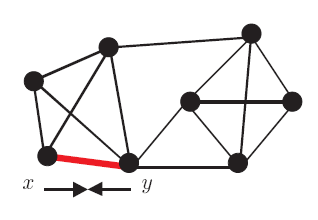
\includegraphics[width=\textwidth]{./images/contract-original-graph.png}
             \caption{Contrazione dell'arco $(x, y)$}
             \label{fig:original-graph}
     \end{subfigure}
   	\hfill
     \begin{subfigure}[b]{0.3\textwidth}
             \centering
             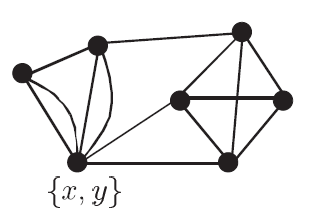
\includegraphics[width=\textwidth]{./images/contract-xy.png}
             \caption{Fusione in un vertice}
             \label{fig:contract-xy}
     \end{subfigure}
    \hfill
     \begin{subfigure}[b]{0.3\textwidth}
             \centering
             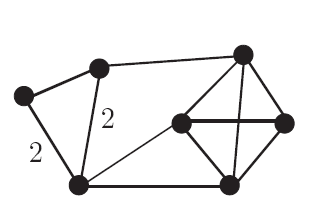
\includegraphics[width=\textwidth]{./images/after-contraction.png}
             \caption{Dopo la contrazione}
             \label{fig:after-contraction}
     \end{subfigure}
     \caption{Esempio di contrazione}
     \label{fig:contraction-example}
\end{figure}

\subsection{Analisi probabilistica}
\label{sub:karger-success-probability}

Per studiare la probabilità di successo per l'algoritmo di Karger ci baseremo sulla seguente proprietà:

\begin{prop}
Sia $ G = (V, E) $ un multi-grafo con $ \lvert V \rvert = n$. Se $G$ ha un min-cut di cardinalità $t$, allora $\lvert E \rvert = \dfrac{t * n}{2}$
\end{prop}

A questo punto dobbiamo calcolare qual'è la probabilità di successo di un'esecuzione di full-contraction, ossia qual'è la probabilità che essa restituisca il taglio minimo del grafo.
Sia $E_{i}$ la probabilità che al passo i-esimo della full-contraction la scelta casuale non seleziona un arco del min-cut:

$$Pr(E_{1}) \geq 1-\dfrac{t}{t n/2}$$
$$Pr(E_{2} \mid E_{1}) \geq 1-\dfrac{t}{t (n-1)/2}$$
$$...$$
$$Pr(E_{i} \mid E_{1} \cup E_{2} \cup ... \cup E_{i-1}) \geq 1-\dfrac{t}{t (n-i+1)/2} = 1 - \dfrac{2}{n-i+1}$$

Ora, la probabilità che ad ogni iterazione non venga scelto un lato del min-cut è:

$$Pr(\bigcap_{i=1}^{n-2} E_{i}) \geq \prod_{i=1}^{n-2} (1 - \dfrac{2}{n-i+1}) = \dfrac{2}{n(n-1)} \geq \dfrac{2}{n^2}$$

\noindent Come possiamo notare questa probabilità è abbastanza bassa. Tuttavia se consideriamo ora la probabilità dell'evento complementare, ossia la probabilità che la nostra procedura di full-contraction non restituisca il taglio minimo del grafo e rieseguiamo la procedura per k volte, essendo ogni esecuzione indipendente, otteniamo:
$$ Pr(\text{le k full-contraction non accumulano la taglia del min-cut}) \leq \left( 1- \dfrac{2}{n^2} \right) ^k $$

\noindent scegliendo pertanto

$$ k = d * \dfrac{n^2}{2} * \log{n} $$

\noindent otteniamo
$$ Pr(\text{le k full-contraction non accumulano la taglia del min-cut}) \leq \left( \dfrac{1}{n^d} \right) $$

\noindent infatti

$$\left( \left( 1-\frac{2}{n^2} \right) ^{\frac{n^2}{2}} \right) ^{\ln {n^d}} \leq e^{-\ln n^d} = \dfrac{1}{n^d}$$

\noindent che è proprio quello che volevamo dimostrare, ossia scelto k in questo modo, l'algoritmo di Karger è corretto in alta probabilità.\\

\noindent $d$ è una costante che permette di abbassare la probabilità di fallimento dell'algoritmo di Karger, infatti più $d$ sarà alto (di conseguenza più elevato sarà k), più sarà bassa la probabilità che l'algoritmo fallisca.




    % \input{chapters/7-tests}
    \section{Estensioni e originalità}
\label{cap:extensions-and-originalities}

\noindent Oltre all'implementazione richiesta dalla consegna
dell'homework, abbiamo deciso di esplorare un altro algoritmo per il problema del taglio minimo.

\subsection{Algoritmo di Karger \& Stein}
\label{sub:karger-stein-algorithm}

L'algortimo di Karger \& Stein è una variante migliorata del semplice algoritmo di Karger. Come abbiamo osservato nella sezione TODO, la probabilità che l'algoritmo di Karger non scelga un arco del taglio minimo tende a diminuire man mano che l'algoritmo durante le iterazione scegli l'arco dove contrarre il grafo. Per questo motico l'algoritmo di Karger \& Stein svolge le prime iterazioni (dove la probabilità di non scelre un arco del min-cut) come l'algoritmo di Karger, mentre le "ultime" iterazioni vengono ripetute più volte con la speranza che qaulcuna di queste non becchi proprio l'arco del min-cut. \\

\noindent Ora supponiamo di volere contrarre gli archi tra n vertici e k vertici in 2 iterazioni di karger normale distinte. Possiamo scegliere a questo punto k in modo da avere una probabilità di successo (ossia di trovare il min-cut) di $\dfrac{1}{2}$. Dunque in questo modo sappiamo che una delle sue esecuzioni indipendenti di Karger avrà successo. Prendiamo quella che ha successo e rieseguiamo tale procedura per il miglior grafo ricavato in una di queste 2 escuzioni. \\

\noindent Se scegliamo k (ossia il numero di iterazioni iniziali) pari a:
$$ k = \dfrac{n}{\sqrt{2}} + 1$$
che equivale a circa il 70\% dei nodi $n$ del grafo rimanenti da contrarre (o equivalentemente abbiamo contratto il 30\% dei nodi $n$ del grafo) a questo punto otteniamo la probabilità desiderata, infatti:

$$ = (1 - \frac{2}{n}) * (1 - \frac{2}{n-1}) * (1 - \frac{2}{n-2}) * ... * (1 - \frac{2}{k+1}) $$

$$ = \dfrac{(1 - \frac{2}{n}) ... (1 - \frac{2}{3})}{(1 - \frac{2}{k}) ... (1 - \frac{2}{3})} = \dfrac{{k\choose 2}^{-1}} {{k\choose 2}^{-1}} = \dfrac{k(k-1)}{n(n-1)}$$

\noindent se inseriamo ora $$ k = \dfrac{n}{\sqrt{2}} + 1$$ otteniamo:
$$ ... = \dfrac{k(k-1)}{n(n-1)} = \dfrac{(\dfrac{n}{\sqrt{2}} + 1) (\dfrac{n}{\sqrt{2}} + 1 - 1)}{n(n-1)} = (\dfrac{\dfrac{n^2}{2} + \dfrac{n}{\sqrt{2}}}{n^2 - n}) \geq \dfrac{1}{2}$$

\noindent come desiderato.\\

\noindent Pertanto l'algoritmo di Karger \& Stein è così formato:
\begin{enumerate}
    \item \textbf{Step 1}: Se $n <= 6$ esegui l'algoritmo di Karger normale stimando il parametro k come visto sopra;
    \item \textbf{Step 2a}: Altrimenti esegui 2 esecuzioni indipendenti di Karger fino a raggiungere $\frac{n}{\sqrt{2}}$ vertici;
    \item \textbf{Step 2b}: Prendi il miglior risultato di queste due esecuzioni e riesegui la seguente procedura.
\end{enumerate}

Il listato \ref{listing:karger&stein} contiene la nostra implementazione di questo algoritmo.


\begin{listing}[!ht]
\begin{minted}{c++}
// kager_stein.h
[[nodiscard]] size_t fast_min_cut(const std::shared_ptr<AdjacencyMapGraph>& graph)
noexcept {
    const size_t n = graph->size();

    // Step 1
    if (n <= 6) {
        const size_t k = utils::estimate_iterations_karger(n);
        return karger(graph, k);
    }

    // Step 2a
    const size_t t =
        static_cast<size_t>(std::ceil((static_cast<double>(n) / std::sqrt(2))));

    auto g1 = full_contraction(graph, t);
    auto g2 = full_contraction(graph, t);


    // Step 2b
    return std::min(fast_min_cut(std::move(g1)), fast_min_cut(std::move(g2)));
}
\end{minted}
\caption{Implementazione dell'algoritmo di Karger \& Stein.}
\label{listing:karger&stein}
\end{listing}


\subsubsection{Successo con alta probabilità e complessità}
\label{sub:karger-stein-success-whp}

Per cominciare calcoliamo il nuovo tempo di esecuzione per una singola iterazione:
$$T(n) = 2T(\dfrac{n}{\sqrt{2}}) + O(n^2) $$
Dal Teorema Master deduciamo quindi che $T(n) = O(n^2 \log{n})$\\

\noindent Possiamo ora quindi scrivere una relazione ricorrente per il successo in probabilità. Sappiamo che la probabilità di successo nelle contrazioni da n a $\dfrac{n}{\sqrt{2}} + 1$ non è più piccola di $\frac{1}{2}$, dunque:
$$P(n) \geq 1-(1- \frac{1}{2}P(\dfrac{n}{\sqrt{2}}))^2$$
A questo punto si può vedere che usando l'induzione: $P(n)= \Omega(\frac{1}{\log{n}}) $. Dunque se facciamo $O(\log^2{n})$ esecuzioni la probabilità di successo e almeno $1-\dfrac{1}{poly(n)}$. Dunque, il tempo di esecuzione totale di questo algoritmo è di:

$$O(n^2 \log^3{n})$$

\subsection{Confronto con KargerMinCut}

\noindent L'algoritmo di Karger \& Stein è nettamente più veloce rispetto all'algoritmo di Karger, com'è possibile vedere in figura \ref{fig:karger-vs-karger-stein}. Basti pensare che eseguire KargerMinCut su tutti e 40 le istanze del dataset richiede circa 2 ore sul computer usato per i benchmark, mentre KargerSteinMinCut richiede circa 2 minuti. Per le istanze a disposizione, l'algoritmo di Karger \& Stein è quindi circa 60 volte migliore di Karger.

\begin{figure}[H]
    \centering

    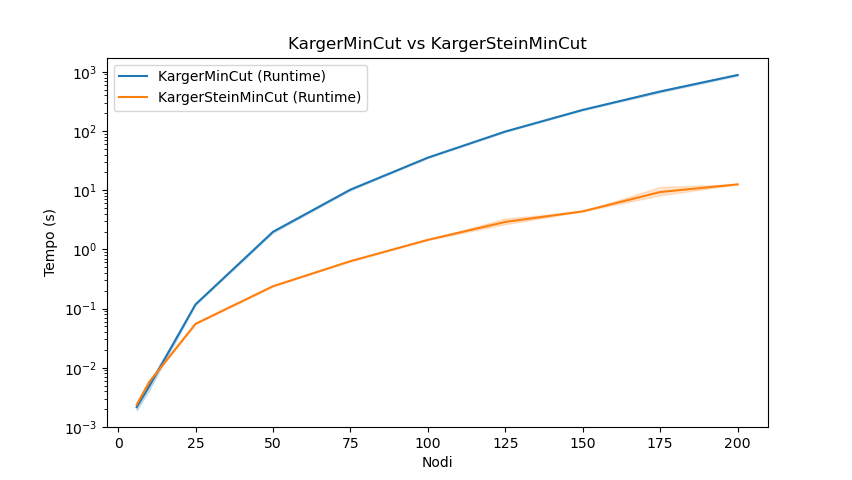
\includegraphics[width=0.9\textwidth]{./images/karger_vs_karger_stein - log.png}

    \caption{Confronto del tempo di esecuzione (in secondi) di Karger \& Stein rispetto a Karger. Grafico in scala logaritmica.}
    \label{fig:karger-vs-karger-stein}
\end{figure}

\subsection{Confronto con KargerMinCutTimeout}

\noindent Chiaramente la differenza di tempi di esecuzione i due algoritmi si riduce se si confronta Karger \& Stein con Karger con timeout $T = 2$ minuti . Come si evince dalla linea piatta in alto a destra di Figura \ref{fig:karger-timeout-vs-karger-stein}, le istanze con più di 150 nodi richiederebbero più di 2 minuti di esecuzioni, quindi l'algoritmo di Karger viene terminato prematuramente.

\begin{figure}[H]
    \centering

    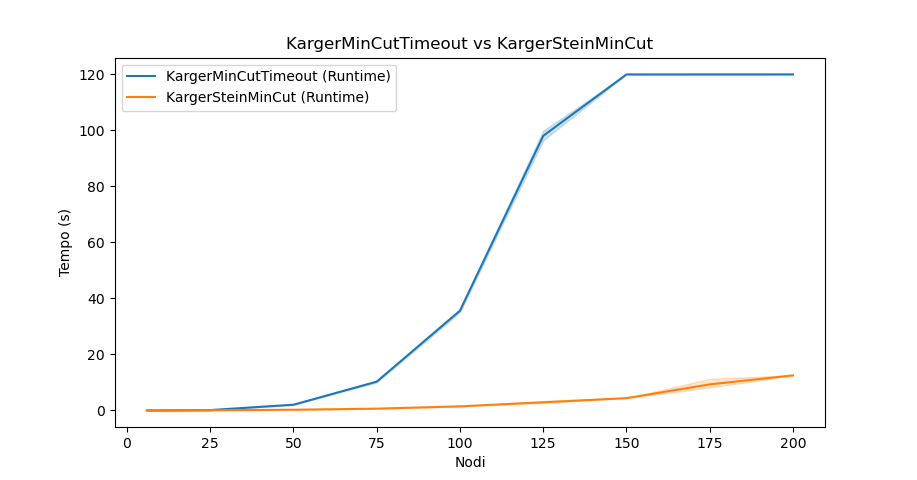
\includegraphics[width=0.9\textwidth]{./images/karger_timeout_vs_karger_stein.png}

    \caption{Confronto del tempo di esecuzione (in secondi) di Karger \& Stein rispetto a Karger con timeout $T = 2 \text{minuti}$.}
    \label{fig:karger-timeout-vs-karger-stein}
\end{figure}

% \ref{table:karger-stein-running-time}


    \section{Analisi dei risultati}
\label{cap:performance-analysis}

\subsection{Domanda \#1}
\label{sec:question-1}

\begin{displayquote}
Misurate i tempi di calcolo della procedura
\codeinline{full\_contraction} sui grafi del dataset. Mostrate i
risultati con un grafico che mostri la variazione dei tempi di calcolo
al variare del numero di vertici nel grafo. Confrontate i tempi
misurati con la complessità asintotica di
\codeinline{full\_contraction}.
\end{displayquote}

\noindent La figura \ref{fig:karger-full-contraction-chart} mostra la
variazione dei tempi di calcolo al variare del numero dei vertici del
grafo ed evidenzia la differenza del tempo di esecuzione pratico di
\codeinline{full\_contraction} rispetto a quello asintotico. È possibile vedere che nella pratica \codeinline{full\_contraction} cresce un po' meno che quadraticamente rispetto al numero di nodi. La tabella \ref{table:karger-full-contraction} mostra invece
un dettaglio di quanto illustrato dal grafico.

\begin{figure}[ht]
    \centering

    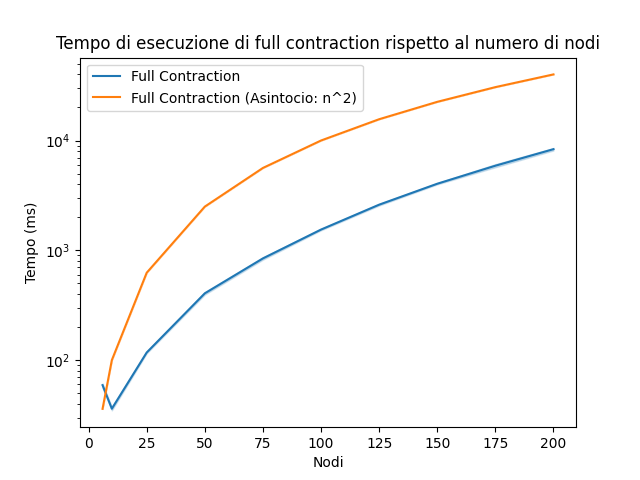
\includegraphics[width=0.9\textwidth]{./images/Tempo_di_esecuzione_di_full_contraction_rispetto_al_numero_di_nodi.png}

    \caption{Confronto tra il tempo di esecuzione di \codeinline{full\_contraction} (in millisecondi) e la sua complessità asintotica rispetto al numero di nodi.}
    \label{fig:karger-full-contraction-chart}
\end{figure}

\subsection{Domanda \#2}
\label{sec:question-2}

\begin{displayquote}
Misurate i tempi di calcolo dell'algoritmo di Karger sui grafi del
dataset, usando un numero di ripetizioni che garantisca una
probabilità minore o uguale a $\frac{1}{n}$ di sbagliare. Mostrate i
risultati con un grafico che mostri la variazione dei tempi di calcolo
al variare del numero di vertici nel grafo. Confrontate i tempi
misurati con la complessità asintotica dell'algoritmo. \\

\noindent Nelle istanze più grandi, il tempo di calcolo necessario a
completare tutte le iterazioni potrebbe risultare eccessivo. In questo
caso utilizzate un timeout oppure abbassate il numero di ripetizioni
per ottenere tempi di esecuzione ragionevoli.
\end{displayquote}

\noindent Per permettere all'algoritmo di Karger un probabilità di
fallimento $ \leq \frac{1}{n}$ è necessario che $d = 1$ e di
conseguenza ricavare $k$ con la formula vista nella sezione
\ref{sub:karger-success-probability}. Quindi:
$$ k = 1 * \frac{n^2}{2} * ln(n)$$

\noindent La figura \ref{fig:karger-runtime-chart} mostra il tempo di
esecuzione (in millisecondi) dell'algoritmo di Karger e lo confronta con il tempo asintotico rispetto al numero di nodi.In questo caso, possiamo notare che la curva teorica e la curva del tempo di esecuzione effettiva sono molto simili, a meno di leggere oscillazioni osservabili soprattutto nei grafi col minor numero di nodi.

\begin{figure}[ht]
    \centering

    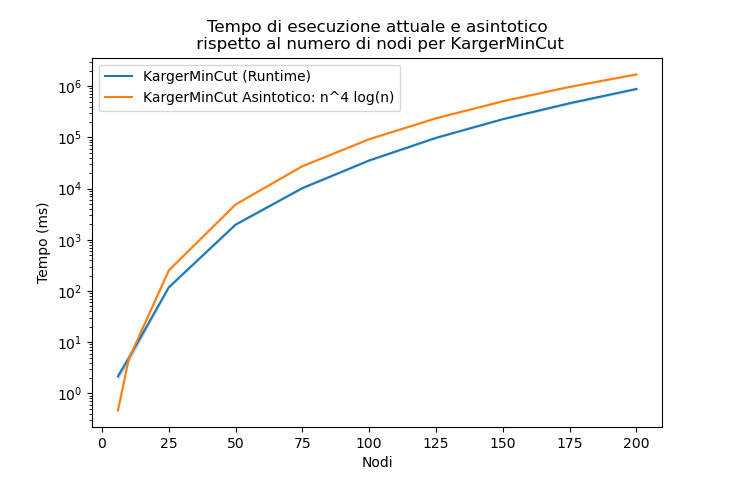
\includegraphics[width=0.9\textwidth]{./images/Tempo_di_esecuzione_attuale_e_asintotico__rispetto_al_numero_di_nodi_per_KargerMinCut.png}

    \caption{Tempo di esecuzione attuale e asintotico per KargerMinCut rispetto al numero di nodi. Grafico in scala logaritmica.}
    \label{fig:karger-runtime-chart}
\end{figure}

\subsection{Domanda \#3}
\label{sec:question-3}

\begin{displayquote}
Misurate il \textit{discovery time} dell'algoritmo di Karger sui grafi
del dataset. Il discovery time è il momento (in secondi) in cui
l'algoritmo trova per la prima volta il taglio di costo mimimo.
Confrontate il discovery time con il tempo di esecuzione complessivo
per ognuno dei grafi nel dataset.
\end{displayquote}

\noindent La figura \ref{fig:karger-discovery-vs-program-time-chart}
mostra un confronto per il \emph{runtime}, ovvero il tempo totale di
esecuzione dell'algoritmo e \emph{discovery time}, ovvero il tempo in
cui l'algoritmo trova il taglio di costo minimo per la prima volta.
Le tabelle \ref{table:karger-running-time} e
\ref{table:kargertimeout-running-time} mostrano il dettaglio dei
dati. \\

\noindent È possibile notare che per la curva di \emph{discovery time}
i risultati hanno molta varianza, ma in linea generale essa è almeno un ordine di grandezza più bassa rispetto a quella del \emph{runtime}. Possiamo ipotizzare che se lanciassimo Karger su grafi di 400 o 1000 nodi, la differenza tra il \emph{discovery time} e il \emph{runtime} sarebbe ancora più evidente. \\

\noindent Ovviamente, come ci si può aspettare, la curva
\emph{discovery time} è considerevolmente più bassa rispetto all'altra
in quanto, data la scelta randomica, ``la volta fortunata'' potrebbe
capitare anche prima della fine dell'algoritmo, e anzi, spesso è così.

\begin{figure}[ht]
    \centering

    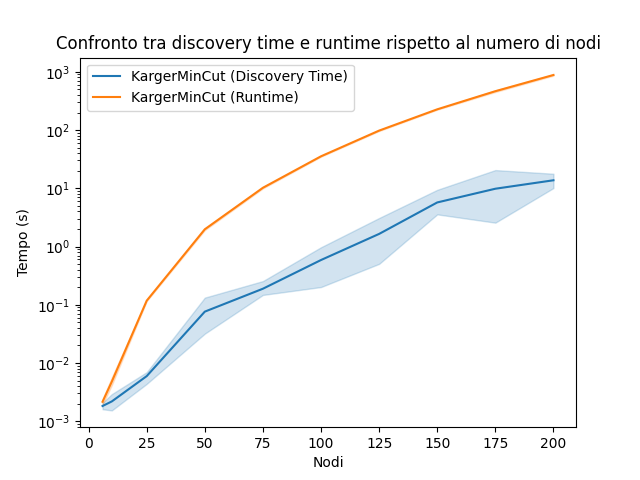
\includegraphics[width=0.9\textwidth]{./images/Confronto_tra_discovery_time_e_runtime_rispetto_al_numero_di_nodi.png}

    \caption{Confronto tra il tempo di esecuzione per \emph{discovery time} e \emph{runtime} rispetto al numero di nodi. Grafico in scala logaritmica.}
    \label{fig:karger-discovery-vs-program-time-chart}
\end{figure}

\noindent La figura \ref{fig:karger-discovery-vs-estimated-k-chart} invece
illustra una comparativa tra il numero di iterazioni tramite le quali
si trova il min cut e il numero di iterazioni $k$ stimato.

\begin{figure}[!ht]
    \centering

    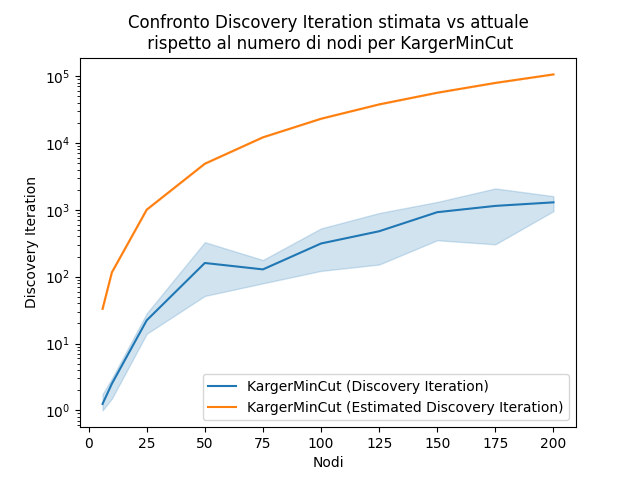
\includegraphics[width=0.9\textwidth]{./images/Confronto_Discovery_Iteration_stimata_vs_attuale__rispetto_al_numero_di_nodi_per_KargerMinCut.png}

    \caption{Confronto discovery iteration stimata vs ottenuta rispetto al numero di nodi per KargerMinCut. Grafico in scala logaritmica.}
    \label{fig:karger-discovery-vs-estimated-k-chart}
\end{figure}

\subsection{Domanda \#4}
\label{sec:question-4}

\begin{displayquote}
Per ognuno dei grafi del dataset, riportate il risultato
ottenuto dalla vostra implementazione, la soluzione attesa e l'errore
relativo calcolato come:

\begin{equation*}
    \frac{SoluzioneTrovata - SoluzioneAttesa}{SoluzioneAttesa}
\end{equation*}

\end{displayquote}

\noindent La nostra implementazione e la scelta del numero di
contrazioni da eseguire non introduce nessun tipo di errore per
l'algoritmo di Karger, quindi un grafico sarebbe poco informativo.\\

\noindent Si ritiene utile invece mostrare le differenza tra
KargerMinCut e KargerMinCutTimeout. Il secondo
differisce dal primo solo perché ad un certo punto l'esecuzione viene
interrotta se l'algoritmo non è ancora terminato.\\

\noindent Dal grafico \ref{fig:karger-vs-kargertout-error-chart} e dal
dettaglio riportato nelle tabelle \ref{table:karger-approx-error} e
\ref{table:kargertimeout-approx-error} è possibile vedere che entrambi
hanno bassissimo errore relativo sull'output, ma Karger impega un
tempo considerevolmente maggiore per risolvere il problema, mentre
KargerMinCutTimeout riesce con successo ad ottenere zero errore anche
prima dello scadere del timeout. Ciò implica che con
KargerMinCutTimeout potrebbe essere utilizzato per avere una soluzione
approssimata entro un tempo accettabile. Quanto descritto è mostrato
nel grafico \ref{fig:karger-vs-kargertout-runtime-chart}.

\begin{figure}[H]
    \centering

    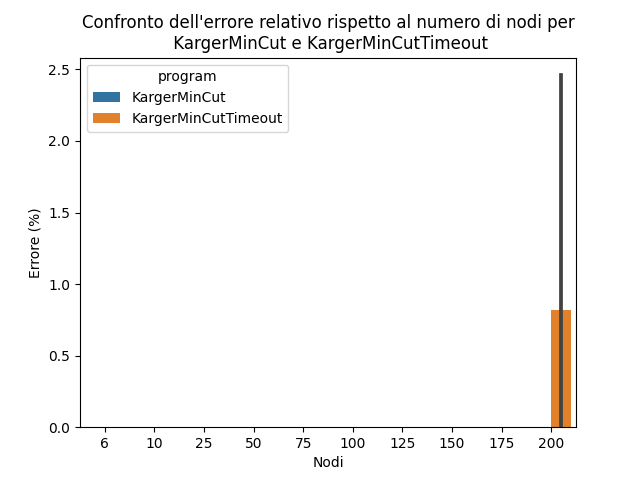
\includegraphics[width=0.9\textwidth]{./images/Confronto_dell'errore_relativo_rispetto_al_numero_di_nodi_per__KargerMinCut_e_KargerMinCutTimeout.png}

    \caption{Confronto dell'errore relativo rispetto al numero di nodi per Karger e Karger con Timeout.}
    \label{fig:karger-vs-kargertout-error-chart}
\end{figure}

\begin{figure}[H]
    \centering

    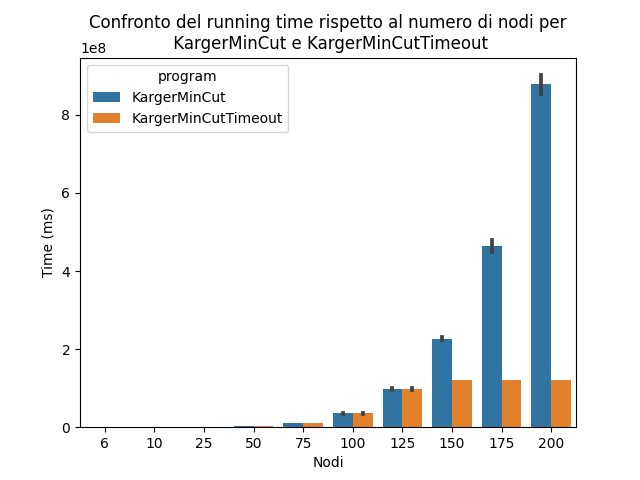
\includegraphics[width=0.9\textwidth]{./images/Confronto_del_running_time_rispetto_al_numero_di_nodi_per__KargerMinCut_e_KargerMinCutTimeout.png}

    \caption{Confronto del running time rispetto al numero di nodi per Karger e Karger con Timeout.}
    \label{fig:karger-vs-kargertout-runtime-chart}
\end{figure}


    \newpage
    \section{Conclusioni}
\label{cap:conclusions}

\noindent Il progetto è disponibile anche come repository pubblica su Github:

\begin{center}
\href{https://github.com/jkomyno/algorithms-hw3}{github.com/jkomyno/algorithms-hw3}
\end{center}


    \newpage
    \appendix
    \section{Tabelle e banchmarks}
\label{cap:tables-and-benchmarks}

\subsection{Tempi di esecuzione}
\label{sec:runtime-tables}

\emph{Nota}: tutti i tempi riportati sono in \textbf{millisecondi}.

\subsubsection{Runtime e Discovery Time}

\begin{table}[H]
    \centering

    \begin{tabular}{lrrr}
     \hline
     \multicolumn{4}{c}{KargerMinCut} \\
     \hline
     Istanza                    &   Nodi &   Discovery Time  &        Runtime \\
     \hline
     input\_random\_1\_6.txt    &       6 &            2.17  &          2.494 \\
     input\_random\_2\_6.txt    &       6 &            1.523 &          1.833 \\
     input\_random\_3\_6.txt    &       6 &            1.753 &          2.104 \\
     input\_random\_4\_6.txt    &       6 &            1.852 &          2.193 \\
     input\_random\_5\_10.txt   &      10 &            3.365 &          6.133 \\
     input\_random\_6\_10.txt   &      10 &            1.591 &          4.272 \\
     input\_random\_7\_10.txt   &      10 &            2.319 &          4.709 \\
     input\_random\_8\_10.txt   &      10 &            1.475 &          4.082 \\
     input\_random\_10\_25.txt  &      25 &            6.326 &        115.6   \\
     input\_random\_11\_25.txt  &      25 &            3.593 &        114.911 \\
     input\_random\_12\_25.txt  &      25 &            7.163 &        122.028 \\
     input\_random\_9\_25.txt   &      25 &            6.706 &        117.197 \\
     input\_random\_13\_50.txt  &      50 &           78.397 &       2036.15  \\
     input\_random\_14\_50.txt  &      50 &          162.461 &       2020.97  \\
     input\_random\_15\_50.txt  &      50 &           20.897 &       1892.18  \\
     input\_random\_16\_50.txt  &      50 &           42.857 &       1956.62  \\
     input\_random\_17\_75.txt  &      75 &          142.054 &       9896.07  \\
     input\_random\_18\_75.txt  &      75 &          169.908 &      10556.8   \\
     input\_random\_19\_75.txt  &      75 &          289.05  &      10387     \\
     input\_random\_20\_75.txt  &      75 &          152.638 &       9979.33  \\
     input\_random\_21\_100.txt &     100 &          915.934 &      35081.1   \\
     input\_random\_22\_100.txt &     100 &          311.953 &      34644.7   \\
     input\_random\_23\_100.txt &     100 &           90.743 &      35958.7   \\
     input\_random\_24\_100.txt &     100 &         1026.61  &      35995.1   \\
     input\_random\_25\_125.txt &     125 &          449.168 &     100097     \\
     input\_random\_26\_125.txt &     125 &          558.167 &      96016.8   \\
     input\_random\_27\_125.txt &     125 &         1647.12  &      98977.3   \\
     input\_random\_28\_125.txt &     125 &         3930.86  &      96256.6   \\
     input\_random\_29\_150.txt &     150 &         4458.47  &     231983     \\
     input\_random\_30\_150.txt &     150 &         3278.94  &     223183     \\
     input\_random\_31\_150.txt &     150 &         3846.83  &     224276     \\
     input\_random\_32\_150.txt &     150 &        11258.7   &     228121     \\
     input\_random\_33\_175.txt &     175 &         7825.21  &     463371     \\
     input\_random\_34\_175.txt &     175 &         3155.08  &     464485     \\
     input\_random\_35\_175.txt &     175 &        26332.9   &     485872     \\
     input\_random\_36\_175.txt &     175 &         1977.07  &     444934     \\
     input\_random\_37\_200.txt &     200 &         7979.94  &     902450     \\
     input\_random\_38\_200.txt &     200 &        18213.6   &     843316     \\
     input\_random\_39\_200.txt &     200 &        16414.2   &     879969     \\
     input\_random\_40\_200.txt &     200 &        12287.4   &     902958     \\
     \hline
    \end{tabular}

    \caption{Runtime e discovery time per KargerMinCut.}
    \label{table:karger-running-time}
\end{table}

\begin{table}[H]
    \centering

    \begin{tabular}{lrrr}
     \hline
     \multicolumn{4}{c}{KargerMinCutTimeout} \\
     \hline
     Istanza                    &   Nodi &   Discovery Time  &        Runtime \\
     \hline
     input\_random\_1\_6.txt    &       6 &            2.073 &          2.839 \\
     input\_random\_2\_6.txt    &       6 &            1.829 &          2.245 \\
     input\_random\_3\_6.txt    &       6 &            2.018 &          2.467 \\
     input\_random\_4\_6.txt    &       6 &            1.98  &          2.47  \\
     input\_random\_5\_10.txt   &      10 &            2.463 &          5.074 \\
     input\_random\_6\_10.txt   &      10 &            2.143 &          4.593 \\
     input\_random\_7\_10.txt   &      10 &            1.947 &          4.758 \\
     input\_random\_8\_10.txt   &      10 &            1.91  &          4.676 \\
     input\_random\_10\_25.txt  &      25 &            6.726 &        113.234 \\
     input\_random\_11\_25.txt  &      25 &            6.449 &        118.174 \\
     input\_random\_12\_25.txt  &      25 &            5.543 &        120.776 \\
     input\_random\_9\_25.txt   &      25 &            4.858 &        114.659 \\
     input\_random\_13\_50.txt  &      50 &          181.982 &       2034.49  \\
     input\_random\_14\_50.txt  &      50 &          307.333 &       2073.14  \\
     input\_random\_15\_50.txt  &      50 &           22.906 &       1982.21  \\
     input\_random\_16\_50.txt  &      50 &           78.742 &       2040.59  \\
     input\_random\_17\_75.txt  &      75 &          661.992 &      10050.1   \\
     input\_random\_18\_75.txt  &      75 &           57.417 &      10652.3   \\
     input\_random\_19\_75.txt  &      75 &          448.759 &      10435.2   \\
     input\_random\_20\_75.txt  &      75 &          193.605 &       9940.02  \\
     input\_random\_21\_100.txt &     100 &          450.032 &      35176.9   \\
     input\_random\_22\_100.txt &     100 &          711.509 &      34926     \\
     input\_random\_23\_100.txt &     100 &          407.518 &      36408.7   \\
     input\_random\_24\_100.txt &     100 &          108.37  &      35952.5   \\
     input\_random\_25\_125.txt &     125 &         1749.07  &     100200     \\
     input\_random\_26\_125.txt &     125 &          392.669 &      96237.8   \\
     input\_random\_27\_125.txt &     125 &         1651.15  &      99110.5   \\
     input\_random\_28\_125.txt &     125 &         2368.78  &      96691.9   \\
     input\_random\_29\_150.txt &     150 &         1983.04  &     120007     \\
     input\_random\_30\_150.txt &     150 &         3466.14  &     120009     \\
     input\_random\_31\_150.txt &     150 &         4788.59  &     120008     \\
     input\_random\_32\_150.txt &     150 &         1387.86  &     120010     \\
     input\_random\_33\_175.txt &     175 &         5307.53  &     120011     \\
     input\_random\_34\_175.txt &     175 &        14102.4   &     120014     \\
     input\_random\_35\_175.txt &     175 &        19510     &     120014     \\
     input\_random\_36\_175.txt &     175 &         3889.23  &     120010     \\
     input\_random\_37\_200.txt &     200 &        22708.9   &     120018     \\
     input\_random\_38\_200.txt &     200 &        38137.8   &     120018     \\
     input\_random\_39\_200.txt &     200 &        21231.2   &     120015     \\
     input\_random\_40\_200.txt &     200 &        32150.5   &     120016     \\
     \hline
    \end{tabular}

    \caption{Runtime e discovery time per KargerMinCutTimeout.}
    \label{table:kargertimeout-running-time}
\end{table}

\subsubsection{Runtime Karger \& Stein}

\begin{table}[H]
    \centering

    \begin{tabular}{lrr}
     \hline
     \multicolumn{3}{c}{KargerSteinMinCut} \\
     \hline
     Istanza                    &   Nodi &       Runtime \\
     \hline
     input\_random\_1\_6.txt    &       6 &      2.48    \\
     input\_random\_2\_6.txt    &       6 &     2.296    \\
     input\_random\_3\_6.txt    &       6 &     2.346    \\
     input\_random\_4\_6.txt    &       6 &     2.354    \\
     input\_random\_5\_10.txt   &      10 &     5.796    \\
     input\_random\_6\_10.txt   &      10 &      5.64    \\
     input\_random\_7\_10.txt   &      10 &     5.745    \\
     input\_random\_8\_10.txt   &      10 &     5.654    \\
     input\_random\_10\_25.txt  &      25 &     54.237   \\
     input\_random\_11\_25.txt  &      25 &     56.346   \\
     input\_random\_12\_25.txt  &      25 &     55.524   \\
     input\_random\_9\_25.txt   &      25 &     54.462   \\
     input\_random\_13\_50.txt  &      50 &    235.358   \\
     input\_random\_14\_50.txt  &      50 &    239.367   \\
     input\_random\_15\_50.txt  &      50 &    238.642   \\
     input\_random\_16\_50.txt  &      50 &    238.475   \\
     input\_random\_17\_75.txt  &      75 &    633.337   \\
     input\_random\_18\_75.txt  &      75 &    630.977   \\
     input\_random\_19\_75.txt  &      75 &    632.557   \\
     input\_random\_20\_75.txt  &      75 &    628.306   \\
     input\_random\_21\_100.txt &     100 &    1456.876  \\
     input\_random\_22\_100.txt &     100 &    1445.885  \\
     input\_random\_23\_100.txt &     100 &    1445.962  \\
     input\_random\_24\_100.txt &     100 &    1434.952  \\
     input\_random\_25\_125.txt &     125 &    2635.854  \\
     input\_random\_26\_125.txt &     125 &    2700.232  \\
     input\_random\_27\_125.txt &     125 &    3525.056  \\
     input\_random\_28\_125.txt &     125 &    2751.982  \\
     input\_random\_29\_150.txt &     150 &    4404.581  \\
     input\_random\_30\_150.txt &     150 &    4385.606  \\
     input\_random\_31\_150.txt &     150 &    4389.538  \\
     input\_random\_32\_150.txt &     150 &    4360.529  \\
     input\_random\_33\_175.txt &     175 &    8217.005  \\
     input\_random\_34\_175.txt &     175 &    8465.02   \\
     input\_random\_35\_175.txt &     175 &   12336.052  \\
     input\_random\_36\_175.txt &     175 &    8162.02   \\
     input\_random\_37\_200.txt &     200 &    12639.06  \\
     input\_random\_38\_200.txt &     200 &   12453.592  \\
     input\_random\_39\_200.txt &     200 &   12532.446  \\
     input\_random\_40\_200.txt &     200 &   12455.888  \\
     \hline
    \end{tabular}

    \caption{Runtime per KargerSteinMinCut.}
    \label{table:karger-stein-running-time}
\end{table}

\subsubsection{Tempi medi di full\_contraction}

\begin{table}[H]
    \centering

    \begin{tabular}{lrrr}
     \hline
     \multicolumn{4}{c}{KargerMinCut} \\
     \hline
     Istanza                    &    Nodi &        Runtime &   Full Contraction \\
     \hline
     input\_random\_1\_6.txt    &       6 &          2.494 &              0.061 \\
     input\_random\_2\_6.txt    &       6 &          1.833 &              0.054 \\
     input\_random\_3\_6.txt    &       6 &          2.104 &              0.06  \\
     input\_random\_4\_6.txt    &       6 &          2.193 &              0.061 \\
     input\_random\_5\_10.txt   &      10 &          6.133 &              0.038 \\
     input\_random\_6\_10.txt   &      10 &          4.272 &              0.036 \\
     input\_random\_7\_10.txt   &      10 &          4.709 &              0.035 \\
     input\_random\_8\_10.txt   &      10 &          4.082 &              0.035 \\
     input\_random\_10\_25.txt  &      25 &        115.6   &              0.116 \\
     input\_random\_11\_25.txt  &      25 &        114.911 &              0.115 \\
     input\_random\_12\_25.txt  &      25 &        122.028 &              0.122 \\
     input\_random\_9\_25.txt   &      25 &        117.197 &              0.116 \\
     input\_random\_13\_50.txt  &      50 &       2036.15  &              0.417 \\
     input\_random\_14\_50.txt  &      50 &       2020.97  &              0.416 \\
     input\_random\_15\_50.txt  &      50 &       1892.18  &              0.389 \\
     input\_random\_16\_50.txt  &      50 &       1956.62  &              0.402 \\
     input\_random\_17\_75.txt  &      75 &       9896.07  &              0.82  \\
     input\_random\_18\_75.txt  &      75 &      10556.8   &              0.873 \\
     input\_random\_19\_75.txt  &      75 &      10387     &              0.858 \\
     input\_random\_20\_75.txt  &      75 &       9979.33  &              0.824 \\
     input\_random\_21\_100.txt &     100 &      35081.1   &              1.529 \\
     input\_random\_22\_100.txt &     100 &      34644.7   &              1.513 \\
     input\_random\_23\_100.txt &     100 &      35958.7   &              1.568 \\
     input\_random\_24\_100.txt &     100 &      35995.1   &              1.569 \\
     input\_random\_25\_125.txt &     125 &     100097     &              2.665 \\
     input\_random\_26\_125.txt &     125 &      96016.8   &              2.554 \\
     input\_random\_27\_125.txt &     125 &      98977.3   &              2.634 \\
     input\_random\_28\_125.txt &     125 &      96256.6   &              2.561 \\
     input\_random\_29\_150.txt &     150 &     231983     &              4.13  \\
     input\_random\_30\_150.txt &     150 &     223183     &              3.973 \\
     input\_random\_31\_150.txt &     150 &     224276     &              3.992 \\
     input\_random\_32\_150.txt &     150 &     228121     &              4.059 \\
     input\_random\_33\_175.txt &     175 &     463371     &              5.874 \\
     input\_random\_34\_175.txt &     175 &     464485     &              5.889 \\
     input\_random\_35\_175.txt &     175 &     485872     &              6.163 \\
     input\_random\_36\_175.txt &     175 &     444934     &              5.645 \\
     input\_random\_37\_200.txt &     200 &     902450     &              8.534 \\
     input\_random\_38\_200.txt &     200 &     843316     &              7.97  \\
     input\_random\_39\_200.txt &     200 &     879969     &              8.318 \\
     input\_random\_40\_200.txt &     200 &     902958     &              8.534 \\
     \hline
    \end{tabular}

    \caption{Tempo medi di esecuzione di \codeinline{full\_contraction} per KargerMinCut.}
    \label{table:karger-full-contraction}
\end{table}

\subsection{Errore di approssimazione}
\label{sec:approx-error-tables}

\begin{table}[H]
    \centering

    \begin{tabular}{lrccc}
     \hline
     \multicolumn{5}{c}{KargerMinCut} \\
     \hline
     Istanza                    &    Nodi &   Min Cut &     Min Cut Atteso &     Errore (\%) \\
     \hline
     input\_random\_1\_6.txt    &       6 &         2 &                  2 &               0 \\
     input\_random\_2\_6.txt    &       6 &         1 &                  1 &               0 \\
     input\_random\_3\_6.txt    &       6 &         3 &                  3 &               0 \\
     input\_random\_4\_6.txt    &       6 &         4 &                  4 &               0 \\
     input\_random\_5\_10.txt   &      10 &         4 &                  4 &               0 \\
     input\_random\_6\_10.txt   &      10 &         3 &                  3 &               0 \\
     input\_random\_7\_10.txt   &      10 &         2 &                  2 &               0 \\
     input\_random\_8\_10.txt   &      10 &         1 &                  1 &               0 \\
     input\_random\_10\_25.txt  &      25 &         6 &                  6 &               0 \\
     input\_random\_11\_25.txt  &      25 &         8 &                  8 &               0 \\
     input\_random\_12\_25.txt  &      25 &         9 &                  9 &               0 \\
     input\_random\_9\_25.txt   &      25 &         7 &                  7 &               0 \\
     input\_random\_13\_50.txt  &      50 &        15 &                 15 &               0 \\
     input\_random\_14\_50.txt  &      50 &        16 &                 16 &               0 \\
     input\_random\_15\_50.txt  &      50 &        14 &                 14 &               0 \\
     input\_random\_16\_50.txt  &      50 &        10 &                 10 &               0 \\
     input\_random\_17\_75.txt  &      75 &        19 &                 19 &               0 \\
     input\_random\_18\_75.txt  &      75 &        15 &                 15 &               0 \\
     input\_random\_19\_75.txt  &      75 &        18 &                 18 &               0 \\
     input\_random\_20\_75.txt  &      75 &        16 &                 16 &               0 \\
     input\_random\_21\_100.txt &     100 &        22 &                 22 &               0 \\
     input\_random\_22\_100.txt &     100 &        23 &                 23 &               0 \\
     input\_random\_23\_100.txt &     100 &        19 &                 19 &               0 \\
     input\_random\_24\_100.txt &     100 &        24 &                 24 &               0 \\
     input\_random\_25\_125.txt &     125 &        34 &                 34 &               0 \\
     input\_random\_26\_125.txt &     125 &        29 &                 29 &               0 \\
     input\_random\_27\_125.txt &     125 &        36 &                 36 &               0 \\
     input\_random\_28\_125.txt &     125 &        31 &                 31 &               0 \\
     input\_random\_29\_150.txt &     150 &        37 &                 37 &               0 \\
     input\_random\_30\_150.txt &     150 &        35 &                 35 &               0 \\
     input\_random\_31\_150.txt &     150 &        41 &                 41 &               0 \\
     input\_random\_32\_150.txt &     150 &        39 &                 39 &               0 \\
     input\_random\_33\_175.txt &     175 &        42 &                 42 &               0 \\
     input\_random\_34\_175.txt &     175 &        45 &                 45 &               0 \\
     input\_random\_35\_175.txt &     175 &        53 &                 53 &               0 \\
     input\_random\_36\_175.txt &     175 &        43 &                 43 &               0 \\
     input\_random\_37\_200.txt &     200 &        54 &                 54 &               0 \\
     input\_random\_38\_200.txt &     200 &        52 &                 52 &               0 \\
     input\_random\_39\_200.txt &     200 &        51 &                 51 &               0 \\
     input\_random\_40\_200.txt &     200 &        61 &                 61 &               0 \\
     \hline
    \end{tabular}

    \caption{Errore di approssimazione di KargerMinCut. Tutte le soluzioni ritornate sono identiche alle relative soluzioni attese.}
    \label{table:karger-approx-error}
\end{table}

\begin{table}[H]
    \centering

    \begin{tabular}{lrccc}
     \hline
     \multicolumn{5}{c}{KargerMinCutTimeout} \\
     \hline
     Istanza                    &    Nodi &   Min Cut &     Min Cut Atteso &     Errore (\%) \\
     \hline
     input\_random\_1\_6.txt    &       6 &         2 &                  2 &           0     \\
     input\_random\_2\_6.txt    &       6 &         1 &                  1 &           0     \\
     input\_random\_3\_6.txt    &       6 &         3 &                  3 &           0     \\
     input\_random\_4\_6.txt    &       6 &         4 &                  4 &           0     \\
     input\_random\_5\_10.txt   &      10 &         4 &                  4 &           0     \\
     input\_random\_6\_10.txt   &      10 &         3 &                  3 &           0     \\
     input\_random\_7\_10.txt   &      10 &         2 &                  2 &           0     \\
     input\_random\_8\_10.txt   &      10 &         1 &                  1 &           0     \\
     input\_random\_10\_25.txt  &      25 &         6 &                  6 &           0     \\
     input\_random\_11\_25.txt  &      25 &         8 &                  8 &           0     \\
     input\_random\_12\_25.txt  &      25 &         9 &                  9 &           0     \\
     input\_random\_9\_25.txt   &      25 &         7 &                  7 &           0     \\
     input\_random\_13\_50.txt  &      50 &        15 &                 15 &           0     \\
     input\_random\_14\_50.txt  &      50 &        16 &                 16 &           0     \\
     input\_random\_15\_50.txt  &      50 &        14 &                 14 &           0     \\
     input\_random\_16\_50.txt  &      50 &        10 &                 10 &           0     \\
     input\_random\_17\_75.txt  &      75 &        19 &                 19 &           0     \\
     input\_random\_18\_75.txt  &      75 &        15 &                 15 &           0     \\
     input\_random\_19\_75.txt  &      75 &        18 &                 18 &           0     \\
     input\_random\_20\_75.txt  &      75 &        16 &                 16 &           0     \\
     input\_random\_21\_100.txt &     100 &        22 &                 22 &           0     \\
     input\_random\_22\_100.txt &     100 &        23 &                 23 &           0     \\
     input\_random\_23\_100.txt &     100 &        19 &                 19 &           0     \\
     input\_random\_24\_100.txt &     100 &        24 &                 24 &           0     \\
     input\_random\_25\_125.txt &     125 &        34 &                 34 &           0     \\
     input\_random\_26\_125.txt &     125 &        29 &                 29 &           0     \\
     input\_random\_27\_125.txt &     125 &        36 &                 36 &           0     \\
     input\_random\_28\_125.txt &     125 &        31 &                 31 &           0     \\
     input\_random\_29\_150.txt &     150 &        37 &                 37 &           0     \\
     input\_random\_30\_150.txt &     150 &        35 &                 35 &           0     \\
     input\_random\_31\_150.txt &     150 &        41 &                 41 &           0     \\
     input\_random\_32\_150.txt &     150 &        39 &                 39 &           0     \\
     input\_random\_33\_175.txt &     175 &        42 &                 42 &           0     \\
     input\_random\_34\_175.txt &     175 &        45 &                 45 &           0     \\
     input\_random\_35\_175.txt &     175 &        53 &                 53 &           0     \\
     input\_random\_36\_175.txt &     175 &        43 &                 43 &           0     \\
     input\_random\_37\_200.txt &     200 &        54 &                 54 &           0     \\
     input\_random\_38\_200.txt &     200 &        52 &                 52 &           0     \\
     input\_random\_39\_200.txt &     200 &        51 &                 51 &           0     \\
     \rowcolor{red!25} input\_random\_40\_200.txt &     200 &        63 &                 61 &           3.279\\
     \hline
    \end{tabular}

    \caption{Errore di approssimazione di KargerMinCutTimeout. Tutte le soluzioni ritornate sono identiche alle relative soluzioni attese, ad eccezione dell'ultima istanza.}
    \label{table:kargertimeout-approx-error}
\end{table}

  \end{document}
